\setcounter{secnumdepth}{1}

\chapter{Lab 2}

\section{Acquisition and Generator}

\begin{Task}{Task 2.1.}
    \textbf{Synchronization} If the clocks of the generator and the acquisition
    are not synchronized, which effect can you expect? Is this equally important for
    low and high frequencies?
\end{Task}

The potential concerns are of 2 kind :
    \begin{itemize}
        \item The first one is the aliasing if the acquisiation clock is slower than the generator clock
        \item The second one is a phase shift between the input and the ouptut which may lead to misleading results for the FRF.
    \end{itemize}

For low frequency signal, those 2 factors are less significant than the case of high frequency signals.

\begin{Task}{Task 2.2.}
    \textbf{Dynamic range} What is the dynamic range of the ADC used
    in the ELVIS II board?
\end{Task}

Considering the ADC got a resolution of 10 bit, the maximum quantization is calculated as follow :
\begin{equation*}
    \text{Quantization} = 2^{10} = 1024 \text{ levels}
\end{equation*}

The LSB is the minimal voltage difference between 2 folliwing voltage measurements.
\begin{equation*}
    \text{LSB} = \frac{V_\text{max}}{1024}
\end{equation*}

This reults as the dynamic range defined as 
\begin{equation*}
    \text{Dynamic range} = 20*log(\frac{V_\text{max}}{\frac{V_\text{max}}{1024}}) = 60 \text{ dB}
\end{equation*}

\section{Sampling}

\begin{Task}{Task 2.3.}
    What is the minimum sampling frequency required to perfectly
    reconstruct a sinusoidal signal with a frequency of 10 Hz?
\end{Task}

Taking the Nyquist limit into account, the sampling frequency should be set at a minimum of 20 Hz.
By security and considering intermodulations/harmonics, the limit is set at 10 times the signal frequency : 100 Hz.

\section{Phase and impact on signal behaviour}

\begin{Task}{Task 2.4.}
    Explain why the accuracy of the FRF is affected by the phase spectrum.
\end{Task}

By only considering the power spectrum of the FRF, we can realize that the time delay / shift introduced by the system between
 the input and the ouptut cannot be taken into account which could result to a misreconstruction of the output time signal.

\begin{Task}{Task 2.5.}
    \textbf{Generation of multisine signals} Use MATLAB to generate the
    data sequence of a multisine that consists of 4096 time samples and contains 100 excited
    spectral lines, located at the low end of the band (from line 1 to 100). Generate
    the multisine with
    \begin{itemize}
        \item (a) a constant phase spectrum
        \item (b) a random phase spectrum, with phases uniformly distributed between [0, 2 pi]
        \item (c) a Schroeder phase spectrum. Choose the phases according to
        \begin{equation*}
            \phi_k = \frac{k(k+1)\pi}{K}
        \end{equation*}
        where k is the line number (= the frequency of the line expressed in bins) and
        K is the number of excited lines in the signal.
    \end{itemize}
\end{Task}

\begin{figure}[H]
    \centering
    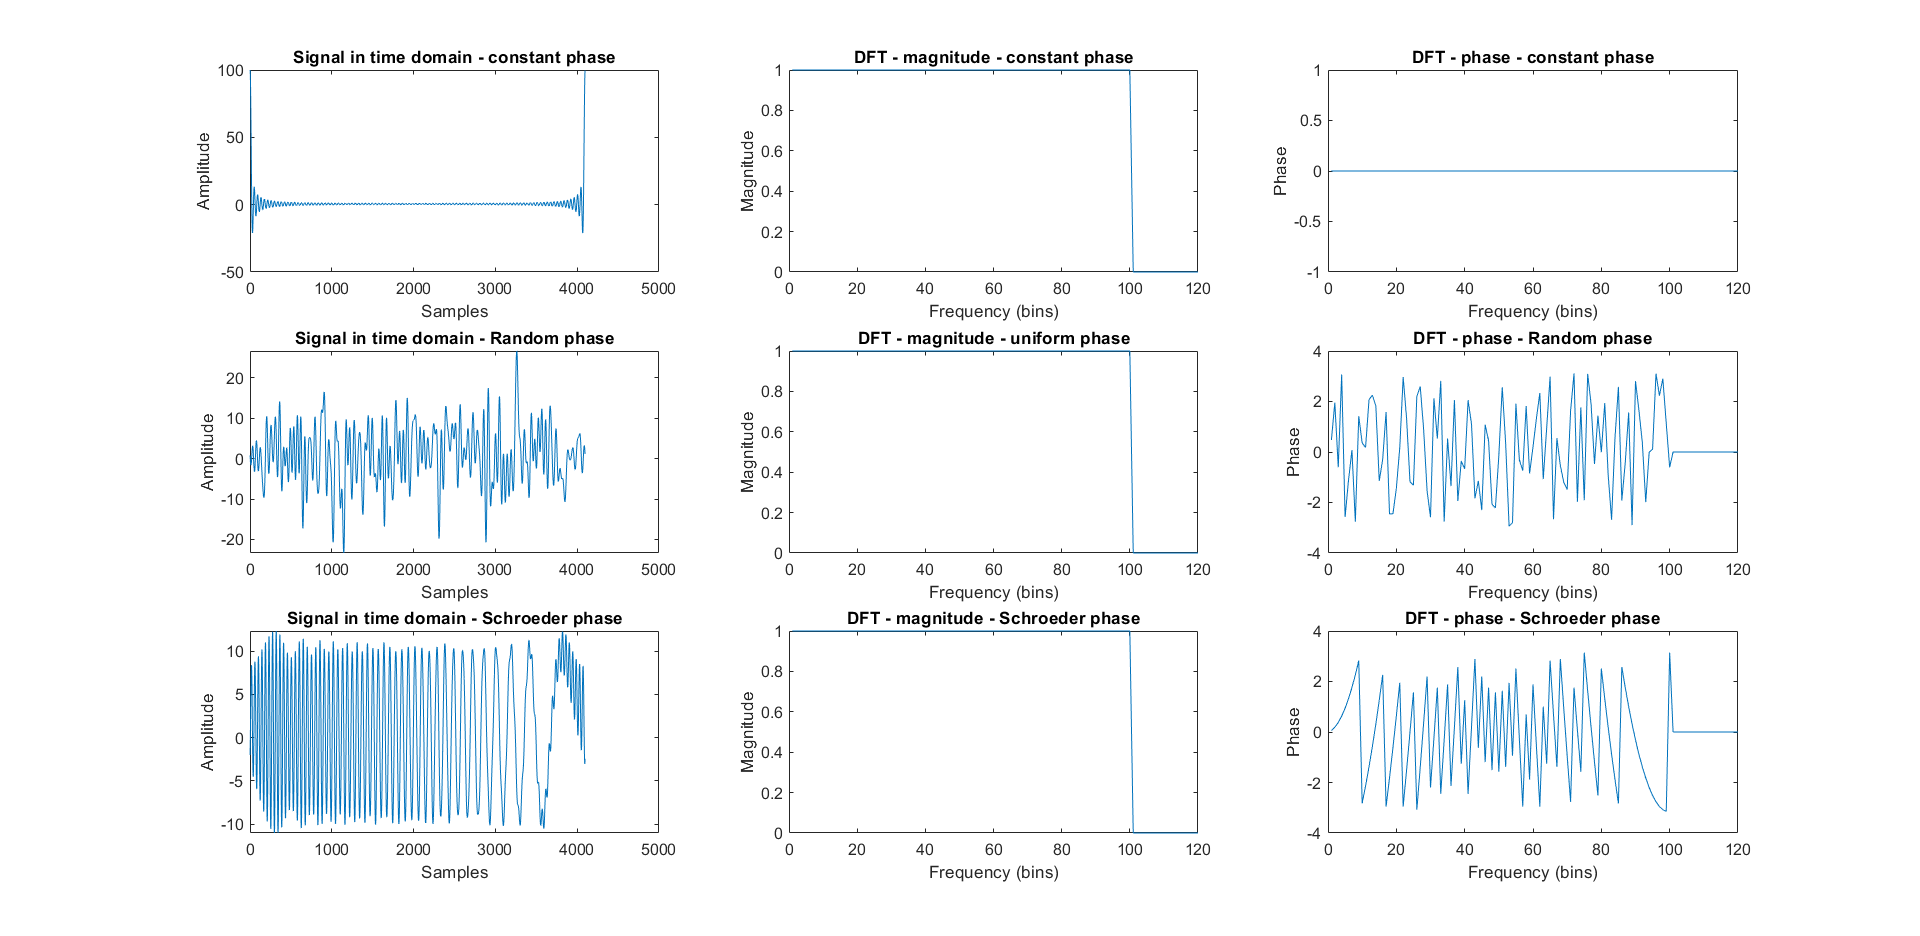
\includegraphics[width=1\textwidth]{Part2/Task_2_5.png}
    \caption{Multisine generation with different types of phase definition}
    \label{Multisine generation}
\end{figure}

\begin{Task}{Task 2.6.}
    \textbf{Crest factor} Calculate the crest factor of these signals and explain
the differences.
\end{Task}

Please find below the crest factor calculated for each signal generation:
\begin{align*}
    \text{Crest factor - constant phase :} 14.072 \\
    \text{Crest factor - random phase :} 3.7526 \\
    \text{Crest factor - Schroeder phase :} 1.7367 \\
\end{align*}

We can see that the random phase signal and the Schroeader phase signal have the lowest crest factor.  This comes from :
\begin{itemize}
    \item (a) Sub-signal phases being desconstructive for the random phase signal resulting to no peak generation in temporal.
    \item (b) Optimized power destribution in temporal domain due to the Schroeder signal definition
\end{itemize}

In contrary, the constant phase signal leads to constructive sub-signals which results to a peak in temporal domain (constructive sub-signals).

\begin{Task}{Task 2.7.}
    \textbf{Plotting and interpretation} Visualize the signals both in the time
    and the frequency domain then discuss differences and similarities.
\end{Task}

Regarding the plot of the signal in temporal and frequency domain, this can be found in the point ~\ref{Multisine generation} 
The interpretation is quite straightforward, the constant phase is genrating sub-signal with the same phase leading the constructive sub-signal reuslting to a peak.
In contrast, the random phase signal and the Schroeder signal are exciting the system with multiple phase signal (please find the DFT plot) leading to a most suitable optmized power distribution.

\section{Transient}

\begin{Task}{Task 2.8.}
    \textbf{Differences between periods} Compare the measurements of the
    different periods of the signal in the time domain and calculate the FRF for each
    period of the signals separately. Explain what you see and decide which periods to
    select or leave out and why.
\end{Task}

The important component to consider while taking the measurement is the response transient.  We should be sure to have enough repetition to 
minimyze the transient component of the signal.  To ensure it, we have to compare the variantion between the current ouput and the previous one.
By comparing the varaition, we filter the output data to keep in order to compute the FRF of the signal.

On the figure below ~\ref{FRF} , we can obeserve the FRF computed at the first repetition and the FRF computed at the 8th one. \\
\textbf{Important note} The varaition of output signal on the figure ~\ref{Time signal response} is highlighted in red.  We can obeserve the variation is more or less the same at
the first repetition and the last one. This may be due to the high reaction speed of the evaluated system meaning that the transient is very small even at the first repetition
 (to be confirmed with the TA).

\begin{figure}[H]
    \centering
    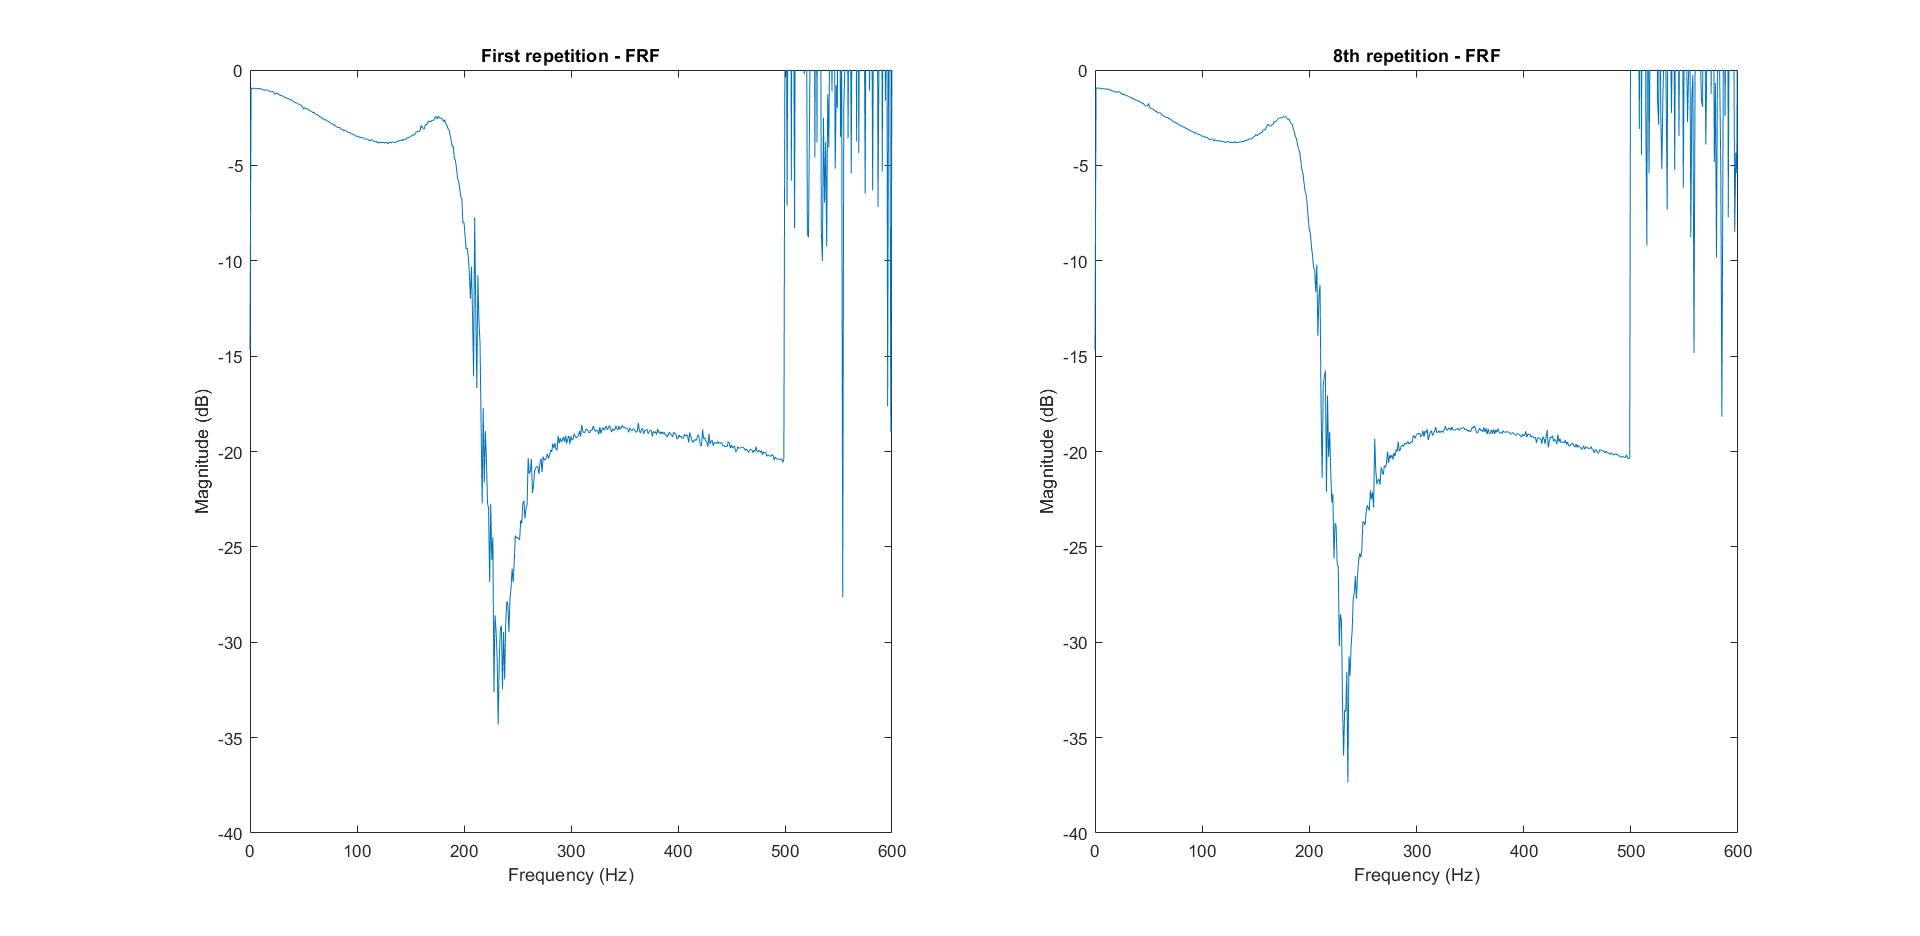
\includegraphics[width=1\textwidth]{Part2/Task_2_7_FRF.png}
    \caption{FRF at the first and 8th repetition}
    \label{FRF}
\end{figure}

\begin{figure}[H]
    \centering
    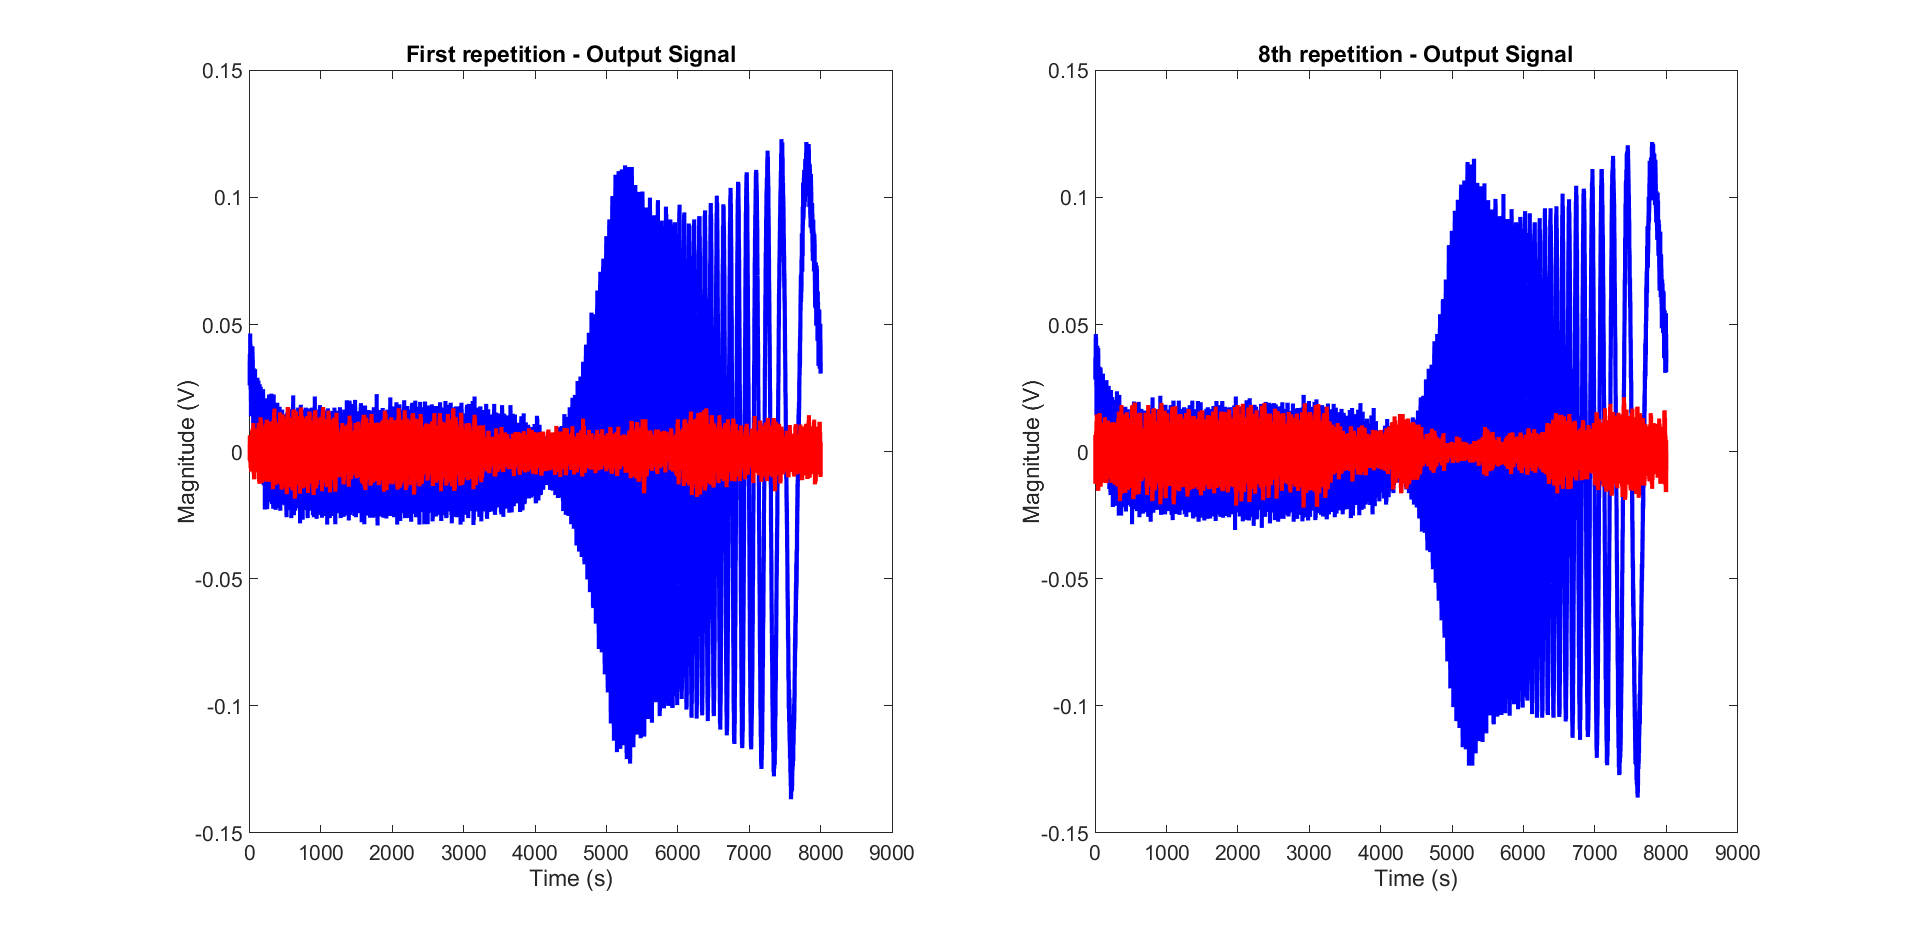
\includegraphics[width=1\textwidth]{Part2/Task_2_7_Output_time.png}
    \caption{Output signal at the first and 8th repetition}
    \label{Time signal response}
\end{figure}

\begin{Task}{Task 2.9.}
    \textbf{Frequency resolution} Visualize the spectra of input and output
    signals. What does this measurement show? Focus on the bandwidth where all the
    important features of the system are included and modify the frequency resolution
    to improve the representation of these features. Fix the frequency resolution for the
    remainder of this lab.
\end{Task}

The figure ~\ref{Power spectrum} shows the power spectrum of the input and the output signal.
We can obeserv easily that the excited band gives us information about the system behaviour at this specific frequency band.
At low frequency, either an very small amplification of the signal or a constant signal power can be observed.  In contrary, at higher frequency, above 150 Hz, we can see a degradation of the signal.
The system behaves like a low pass filter with a cut off at 150 Hz.

\begin{figure}[H]
    \centering
    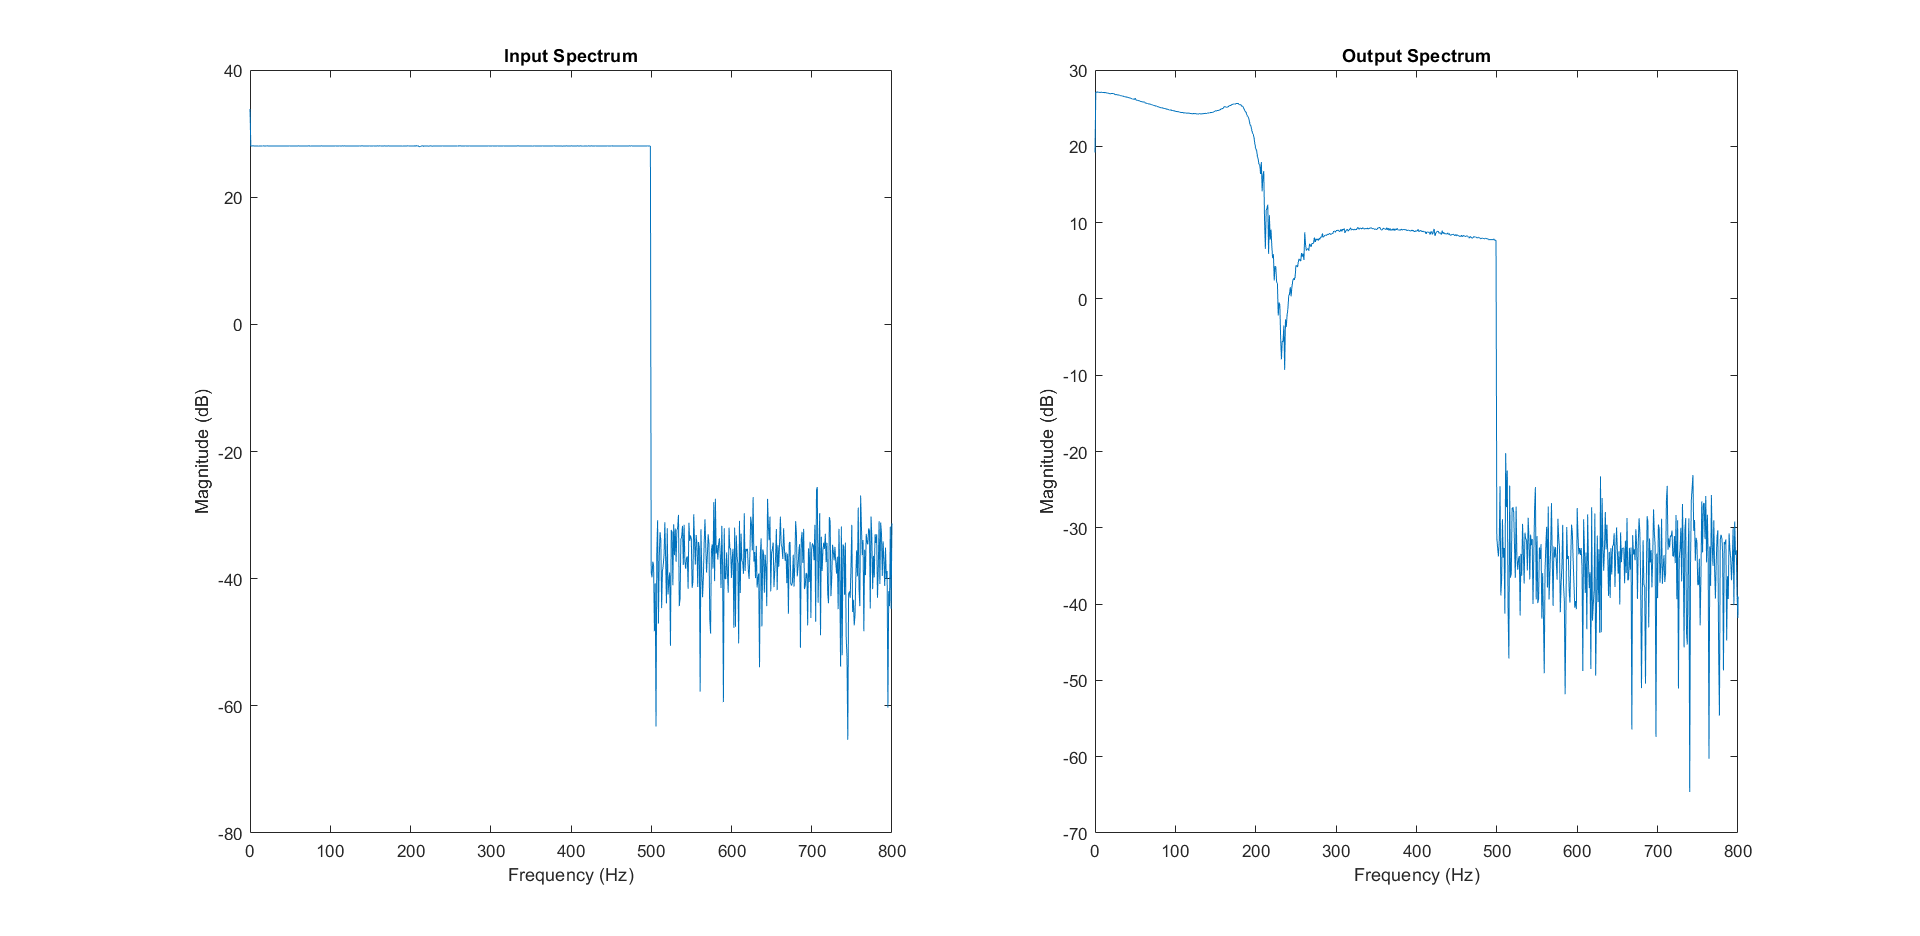
\includegraphics[width=1\textwidth]{Part2/Task_2_9_power_spectrum.png}
    \caption{Power spectrum of the input and output signals}
    \label{Power spectrum}
\end{figure}

\begin{Task}{Task 2.10.}
    \textbf{FRF computation For each measurement} compute the FRF and
    provide a plot in the report. Which differences do you observe? Explain.
    \textbf{Periodic}
    \begin{itemize}
        \item(a) The Schroeder multisine designed in the previous section.
        \item(b) A multisine with constant phase and amplitude in the specified analysis band
        only.
        \item(c) A multisine with an arbitrary (random) phase and constant amplitude in the
        specified analysis band only.
        \item(d) A periodic noise signal.
    \end{itemize}
    \textbf{Aperiodic}
    \begin{itemize}
        \item(e) An aperiodic noise signal. Remember that here measuring P periods requires
        to load P different signals in the AWG.
        \item(f) Same as (e), but multiply the measured aperiodic input and output signals by
        a Hann window and observe the results. How are the results in comparison to
        the results with a rectangular window?
    \end{itemize}
\end{Task}


\textbf{Periodic}

For periodic signals, we can obeserve differences depending on if the signals have constant phase, random phase or schroeder phase.

\begin{itemize}
    \item (a) The constant phase signals lead to a very clean FRF power spectrum.  The cleaniless of the FRF is due to the
    constructive sub-signals (same phase) leading to a high signal power.  The drawback of this excitation is the non-linearity / harmonics 
    distorsion if the system is non-linear (which is not the case of this TP).
    \item (b) The random phase signals lead to a more noisy FRF power spectrum (less sharp).  Nevertheless, this excitation is more robust once
    we deal with system introducing noise or non-linearity (cf Crest factor).
    \item (c) Schroeder phase signals are the most optimiwed signal to compute a clean FRF due to the optimized energy distribution across the frequency band.
    The orthogonal characteristic of the frequency components allow to have no interference between frequencies which would result to distorsion of the FRF.
    \item (d) the periodic noise signal results to the noisiest FRF as excpected due to his random nature.  Nevertheless, by repetiting the signal, the
    FRF computed is still leading to relevant result due to the minimization of the transient after each period.

\end{itemize}

\begin{figure}[H]
    \centering
    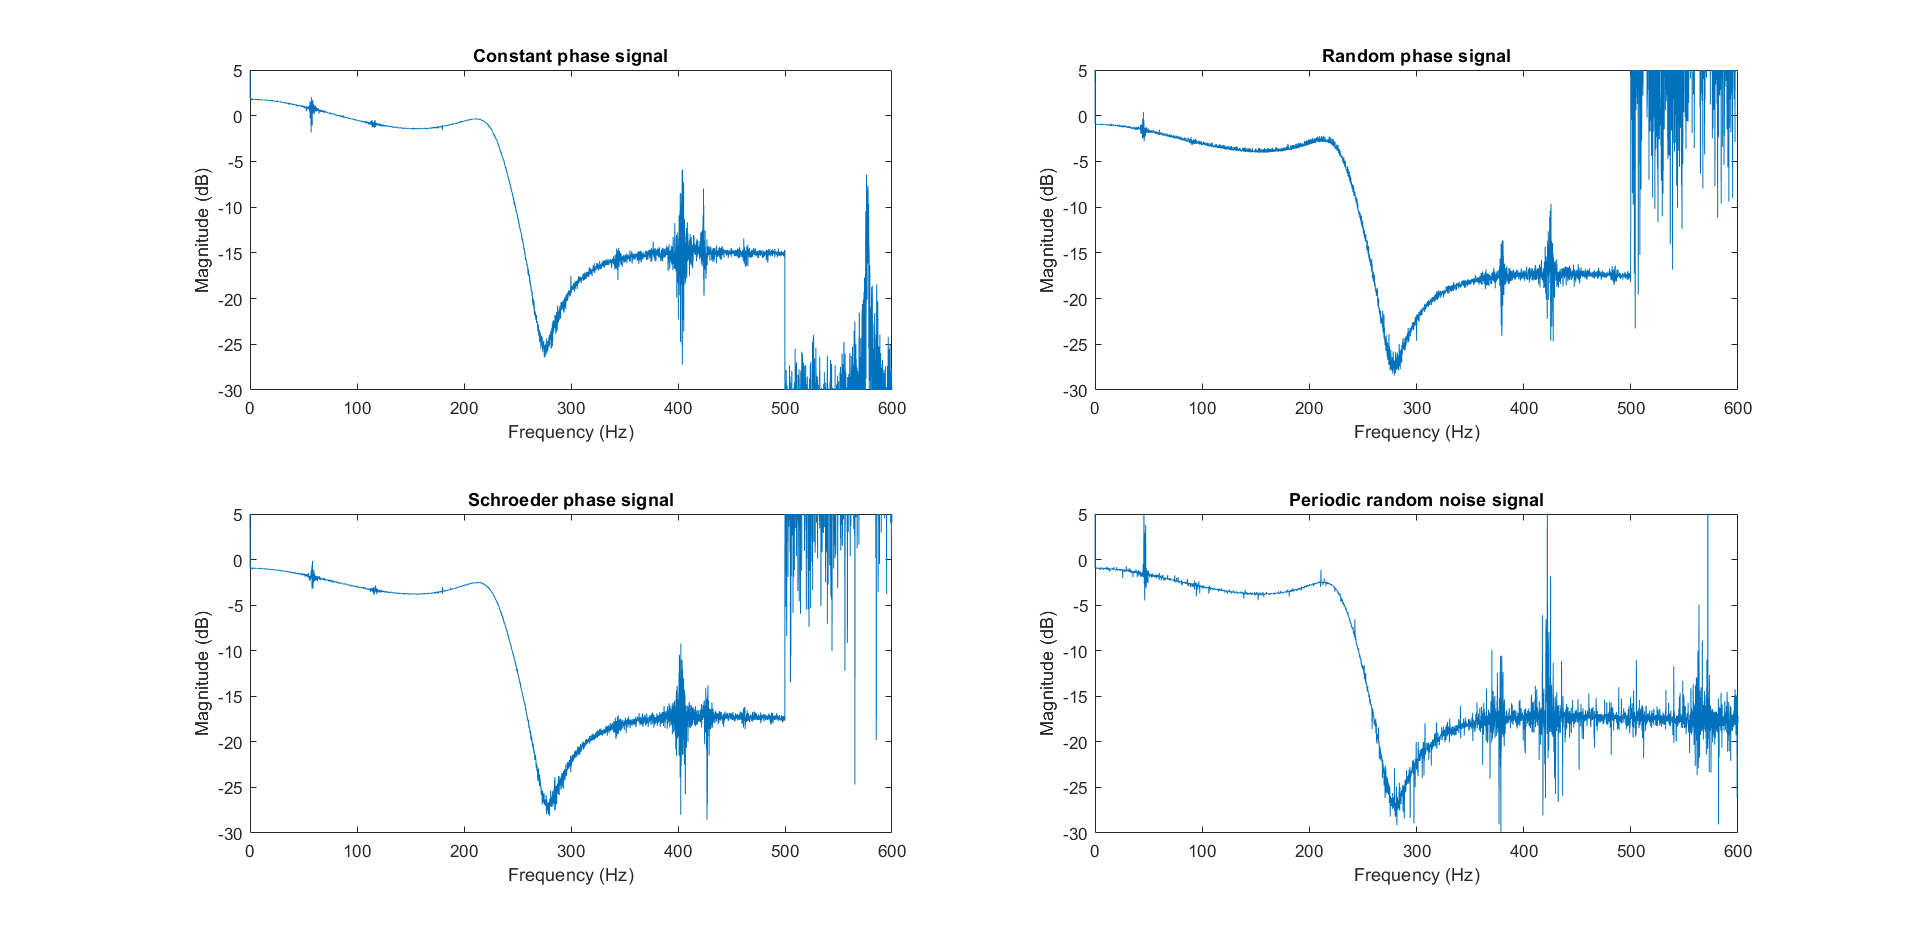
\includegraphics[width=1\textwidth]{Part2/Task_2_10_power_spectrum_periodic.png}
    \caption{Power spectrum of FRF}
    \label{Power spectrum periodic signal}
\end{figure}

\begin{figure}[H]
    \centering
    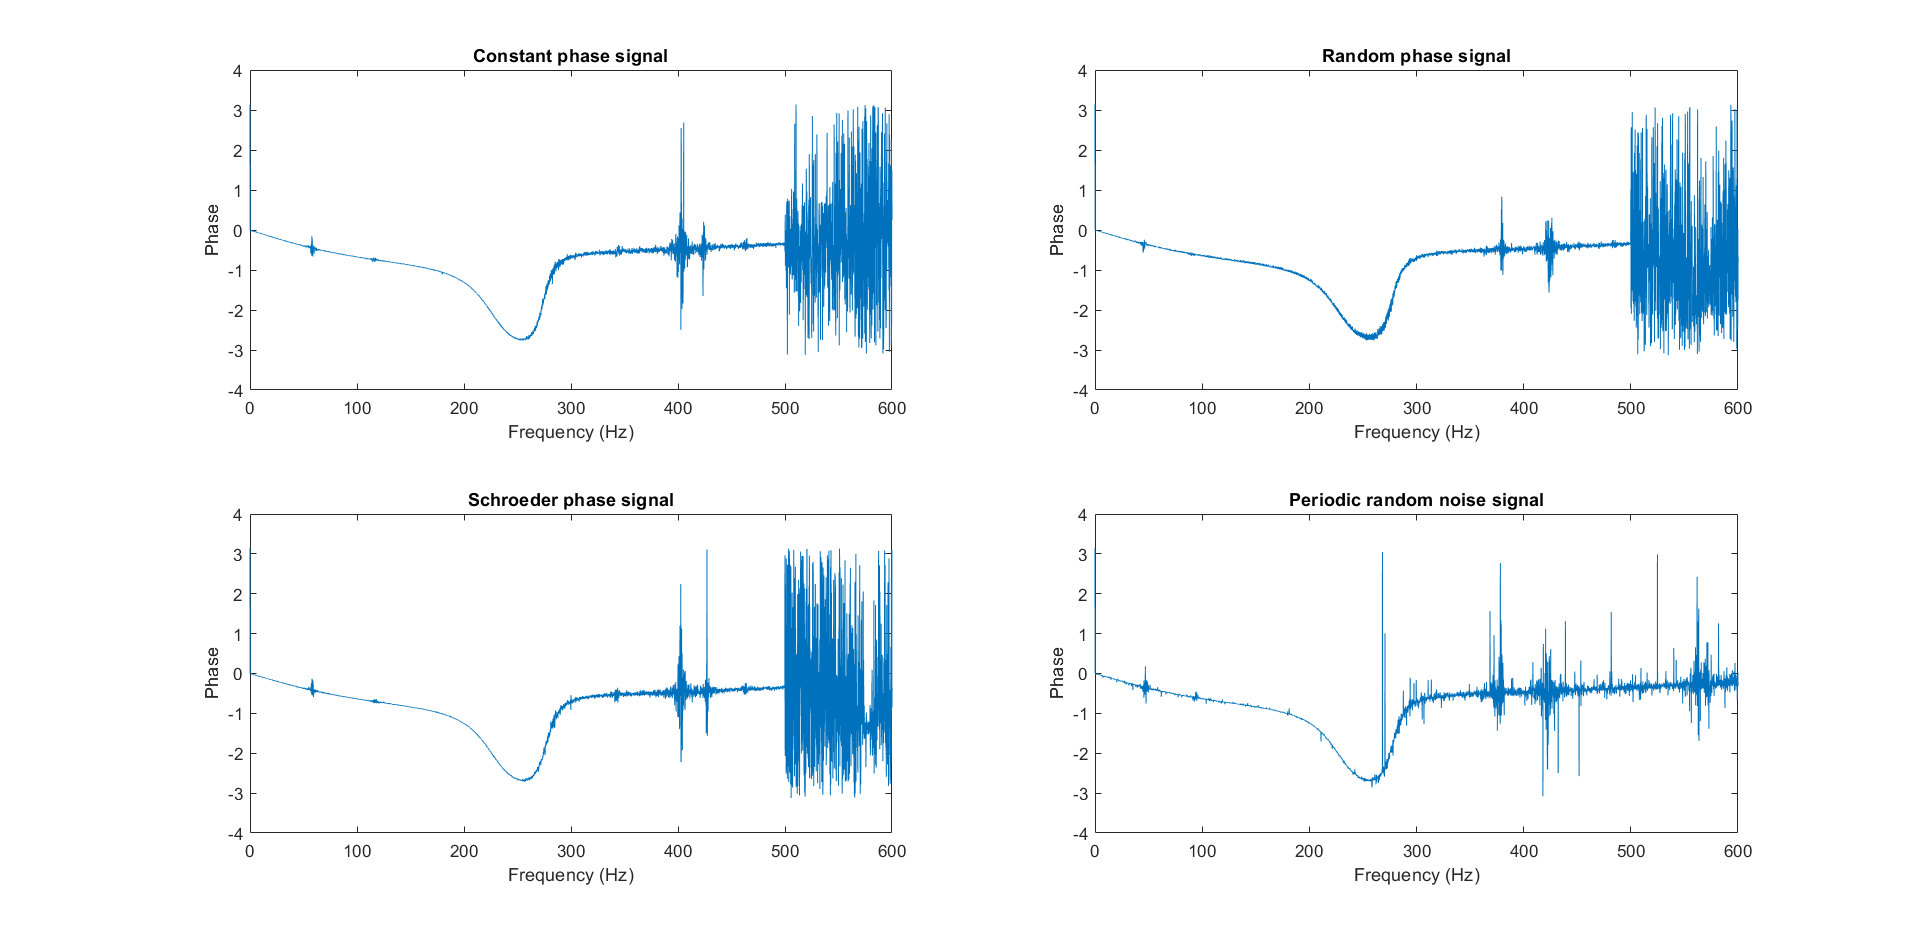
\includegraphics[width=1\textwidth]{Part2/Task_2_10_phase_spectrum_periodic.png}
    \caption{Phase spectrum of FRF}
    \label{Phase spectrum periodic signal}
\end{figure}

\textbf{Aperiodic}

Regarding aperiodic signals, the wrong manipulation leads to invalid results.
Those results will be re-done during week 28.






